\chapter{Исследовательский раздел}

\section{Технические характеристики}

Тестирование производительности программы генерации производилось на компьютере со следующими техническими характеристиками:
\begin{itemize}
	\item операционная система: Ubuntu 19.10 64-bit;
	\item память: 3,8 GiB;
	\item процессор: Intel® Core™ i3-6006U CPU @ 2.00GHz (4 логических ядра).
\end{itemize}

\section{Время заполнения БД фейковыми данными}

На рисунке \ref{img:generate-time} показано время заполнения БД фейковыми данными.
$1000$ пользователей создались за $0,87$ с, $1000$ тэгов — за $0,61$ с, $1000$ статей, в каждой из которых до 15 предложений, — за $2,19$ с, $10000$ комментариев, в каждом из которых до 7 предложений, — за $7,82$ с, до $100$ голосов на каждый пост и до $10$ голосов на каждый пост (сгенерировался $100121$ голос) — за $8,38$ с.

Быстрая генерация данных обеспечена грамотным использованием \code{bulk\_create}.
Высокое качество сгенерированных данных получено благодаря библиотеке \code{Faker} \cite{faker}.

На рисунке \ref{plt:bulk-create} представлена зависимость времени генерации 10000 комментариев от максимального количества предложений в нём.
Видно, что зависимость имеет линейный вид.
Поэтому, для ускорения времени работы генерации, в программе были выделены в параметры командой строки максимальное количество предложений в статье и комментарии.

\begin{figure}[H]
	\centering
	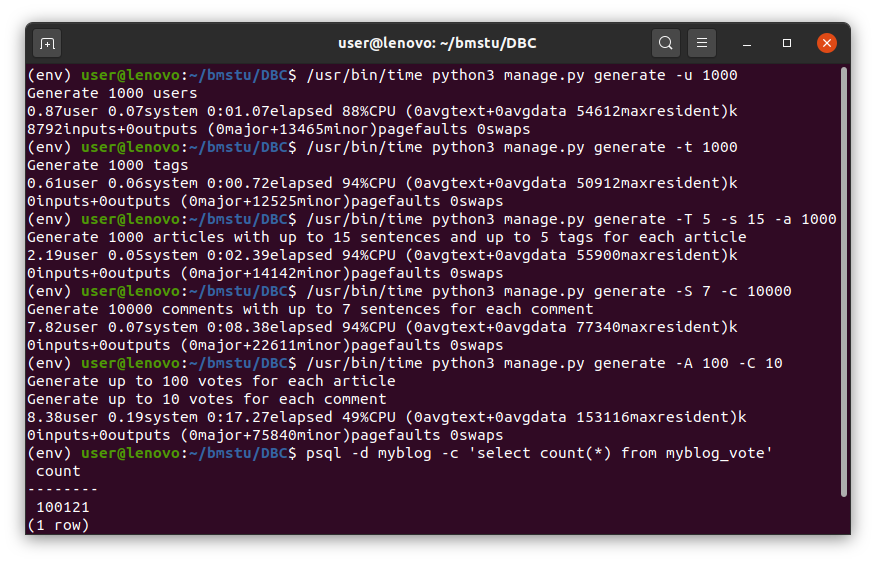
\includegraphics[width=\linewidth]{inc/img/generate-time}
	\caption{Время заполнения БД фейковыми данными}
	\label{img:generate-time}
\end{figure}

\begin{figure}[h!]
	\centering
	\begin{tikzpicture}[scale=0.9]
	\begin{axis}[
		axis lines=left,
		xlabel={Максимальное кол-во предложений},
		ylabel={Время, с},
		ymin=0,
		legend pos=north west,
		ymajorgrids=true
	]
	\addplot table[x=sentences,y=time,col sep=comma]{inc/csv/bulk_create.csv};
	\end{axis}
	\end{tikzpicture}
	\captionsetup{justification=centering}
	\caption{Зависимость времени генерации 10000 комментариев от максимального количества предложений в нём}
	\label{plt:bulk-create}
\end{figure}

\section*{Вывод}

Вставка большого количества данных в таблицу с помощью \code{bulk\_create} происходит довольно быстро.
Для ещё большего ускорения генерации можно уменьшить максимальное количество предложений в каждой статье или комментарии, однако это отрицательно повлияет на качество сгенерированных данных.
